\documentclass[12pt,final]{article}
\usepackage[letterpaper,hmargin=3.5cm,vmargin=3.5cm]{geometry}
\usepackage{graphicx}
\usepackage[labelsep=period,font=small,textfont=bf,labelfont=bf,skip=0.1cm]{caption}
\usepackage[labelformat=simple,labelsep=period,font=small,skip=0.0cm]{subcaption}
\usepackage[authoryear]{natbib}
\usepackage{multirow}
\usepackage{color}
\usepackage{amsmath}
\usepackage{amsfonts}
\usepackage{amssymb}
\usepackage{pdfpages}
\usepackage[title]{appendix}
\setlength{\parskip}{2mm}
\definecolor{myurlcolor}{rgb}{0,0,0.65}
\usepackage[pdftitle={Parra Exp Idea Lying}, pdfauthor={Daniel Parra}, pdfstartview={FitH}, colorlinks=true, hyperfootnotes=false, linkcolor=black, citecolor=black, urlcolor=myurlcolor]{hyperref}
\usepackage{rotating}
\usepackage{booktabs}
\setcounter{secnumdepth}{2} % Levels of section headings that should be numbered
\setlength{\footnotesep}{2.4ex} % Footnote spacing
\renewcommand{\baselinestretch}{1.6}
\newtheorem{result}{Result}
\newtheorem{hypothesis}{Hypothesis}
\newcommand{\mcl}{\multicolumn}
\newcommand{\cc}{\multicolumn{1}{c}}
\newcommand{\s}{\scriptsize}
\newcommand{\h}{\hspace}
\newcommand{\mrw}[1]{\multirow{#1}{*}}
\usepackage{etoolbox}
\usepackage{placeins} %package for creating float barriers 
\AtBeginEnvironment{thebibliography}{\linespread{1}\selectfont}

%%%% no comma between name and year in citations
%\bibpunct{(}{)}{;}{a}{}{,}


\begin{document}
%==============================================================================
%This is the title page
\setcounter{page}{1} \thispagestyle{empty} \renewcommand{\thefootnote}{\fnsymbol{footnote}} %\vspace*\fill %
\phantomsection\addcontentsline{toc}{section}{Business culture}

\begin{center}
\vspace{+0.5cm}%
\huge\textbf{Because I deserve it: endowment effect, loss aversion and lying behavior}% Title
\vspace{+0.5cm} \\ %
\Large{Daniel Parra}\\ \small{WZB Berlin Social Science Center, e-mail: \href{mailto:daniel.parra@wzb.eu}{daniel.parra@wzb.eu}} \\
\end{center}

\begin{abstract}
\noindent his paper presents an experimental design of a cheating game based on the die-roll paradigm \citep{Fischbacher2013}. The design aims to assess whether the endowment effect increases the desire to lie. In particular, we have a baseline and two treatments, in which we have two different kinds of the endowment effect. In one, the endowment is given by the experimenter, and in the other, the endowment is obtained by a real effort task \citep{Benndorf2014}. We hypothesized that the feeling of deserving the endowment would generate a justification to lie, and as a consequence lying will increase.
\end{abstract}

%\vspace*\fill
% First version: May 2012 \\
\indent This version: October 12, 2018

JEL Codes: C91, D02, D90.

Keywords: Cheating, unethical behavior, endowment effect, fairness. \\
\vspace*\fill
%End of title page
%===========================================
%Here the main text starts
\pagebreak \renewcommand{\thefootnote}{\arabic{footnote}} \setcounter{footnote}{0}

\section{Introduction}\label{sec:intro}

Lying is an important issue in society. Several examples of its damage shown how people lie in real life for obtaining some benefits.  Among these cases, we can mention Enron, Lehman Brothers, and Volkswagen. According to \citet{Gneezy2018},  lying is a behavior that occurs when some agent misreports some private information. Laboratory experiments have provided evidence for the fact that people do not lie in a significant extent in the Lab \citep{Abeler}, or at least they do not lie as rationality would predict.

One common experimental paradigm to study lying behavior is the one introduced by \citet{Fischbacher2013}. These authors create a simple game in which participants privately roll a die, and only them can observe the result. Once participants have learned the result,  they must report the outcome; then they will be paid accordingly with the number they report.  Standard economics will predict everyone lying. However, the empirical evidence does not corroborate this prediction. \citet{Abeler} shows that the most plausible explanation is that people when facing the possibility of cheating, have a utility function that combines a preference for being honest with a preference for being seen as honest.


Behavioral economics has shown us that preferences are not well-defined, context independent or stable \citep{Loewenstein2003,Simonsohn2006,Ariely2003,Ariely2006}, therefore if it exists a preference for honesty, it should also have the same limitations than another kind of preferences. In that way, this paper aims to present an experimental design that assesses the impact of a broadly studied bias, the endowment effect \citep{Kahneman2011,Kahneman1991}, on the lying behavior, i.e., on the preferences for truth-telling. A common consequence of the endowment effect, in a market context, is that it makes that measures of willingness to accept greatly exceed measures of willingness to pay. In a cheating context, we could expect that the willingness to lie for keeping money will exceed the willingness to lie for gaining money. Moreover, we also expect that if the endowment is not given but gained through some personal effort, the willingness to lie will be higher.

The way in which we plan to introduce the endowment effect will be with two different treatments. In one we will give money to the participants, and after that, they will have the possibility of lying for keeping some part of it. A second treatment will strengthen the endowment effect by allowing the participants to earn money previously and then report a die-roll for giving back some part of it. The reason to include the second treatment is that it will allow the agent to create justification for lying and could foster cheating. In that way, we can compare the standard set up of the endowment effect and one scenario where participants could have the feeling that they deserve the money and then the intrinsic cost for lying is smaller.

This study will contribute to the understanding of lying behavior, and it will shed some light on the importance of choice architecture on context with potential possibilities to lie. For instance, there are countries with tax systems that make people pay taxes in advance and next year they claim reimbursements, in other systems citizens should declare their incomes, and then they have a bill for the taxes. Then our results could give some advice for policy-makers for creating environments where lying is more difficult. The study also will contribute to the literature of anomalies, in specific it will provide evidence of the impact of the endowment effect \citep{Kahneman2011,Kahneman1991} and loss aversion \citep{Tversky1991} on truth-telling preferences.

The overall structure of this paper takes the form of four sections. The first one is this introduction that presents the aim of the experimental design and its motivation. In the second section, I will present a short related literature on the topics of endowment effect and lying, in order to present the previous relevant studies in which this research is built. The third section is the core of the paper, so it presents the experimental design with the main components as treatments, hypotheses, procedures. Section fourth presents some final remarks.

\section{Related Literature}\label{sec:literature}
First of all, it is important to point out that an in-depth literature review is beyond the scope of this paper, instead, the purpose of this section is to locate our experiment on the closest related literature; for a comprehensive literature review of experimental research on lying see \citet{Rosenbaum2014} and \citet{Abeler}. The experimental research on cheating had used, mainly, three different paradigms: the sender-receiver, the matrix task, and the die roll task. 

\citet{Gneezy2005} introduced the sender-receiver paradigm, where one agent has information about which one of two possible states of the world is the true one. After learning the actual state, he says to a second player which one it is, but he can misreport the state for his own benefit. The advantage of this game is that it allows the experimenter to observe whether the participants lie or not. However, the strategic interaction makes the interpretation less clean. The second paradigm, the matrix task, was presented by \citet{Mazar2008} and is based on a mathematical task where participants should self-report their performance. Before his report, the experimenter destroys the sheet with the matrices solved, so lying is not detectable individually.

The third paradigm, and the most relevant for our experimental design, was introduced by \citet{Fischbacher2013}. In this set-up, participants roll a six-sided die, and then they report the outcome of the die. The payoff would equal 1, 2, 3, 4, or 5 tokens if the die number that they report is the corresponding payoff amount, and 0 tokens if the die number that they report is a 6.  The main advantage of this game is that, as well as \citet{Mazar2008}, it avoids demand effects because the experimenter cannot observer the individual behavior, but we know the real underlying distribution of the outcome if people are honest. Therefore, we have an objective counterfactual as a benchmark for analyzing the results.


In the die-roll paradigm the payoff-maximizing strategy is always to report a 5, i.e., if people care just about money, they should lie to the full extent (report a 5). On the other hand, if people are completely honest, the payoff should follow a uniform distribution with an average of 3, so it should not exist statistical differences. \citet{Fischbacher2013} found that 20\% of the participants lied to the fullest extent possible,  and 39\% behave honestly; hence a significant share of the participants are partial liars.  After this seminal work, several scholars used the die roll paradigm. \citet{Abeler} reports a meta-study that covers 72 experiments where they find that indeed subjects earn on average about a quarter of what they could win with the profit-maximizing strategy. Besides, players are still using the same strategy even when stakes were increased 500-fold.

Nevertheless, \citet{Kajackaite2017a} present evidence in the way that the conclusion that the preference for reporting the truth seems to be insensitive to extrinsic motivation could be misleading. In order to do so, they replicate the finding in previous works, however \citet{Kajackaite2017a} shows that this insensitivity is not a characteristic of the intrinsic lying cost, but rather a result of concern about being exposed as a liar.  Then, they used a "mind" game that consisted of a similar die-roll game, but participants are asked before to think in a number, then they must report if the die that came up is the same number they thought. In this manipulation, the researchers eliminate the concern of being exposed as a liar, as a consequence agents lied more.  This paper implies that people make a cost-benefit analysis where they take into the account the intrinsic costs of lying and the incentives to lie. 

Hence, we can state that incentives are significant in lying contexts, but they need more study to understand the factors that influence the desire to lie; in other words, we need to consider what increases the intrinsic and extrinsic incentives to lie. Nevertheless, regardless of the possible incentives that play a role when deciding whether to lie, what previous scholar had shown is that lying is a complex phenomenon that should be considered with a behavioral perspective rather than with a standard economics perspective. In other words, we need to consider which 
anomalies could change the decision making or could affect the preferences to being honest. 

Provided that behavioral biases could influence preferences for lying/truth-telling, then a well-known anomaly, the endowment effect, could have an impact on it. In particular, our design includes it as the central question because it could give some policy implications on tax schemes. \citet{Thaler1980} was the first scholar that introduced the endowment effect in the economic literature.  Specifically, he define it as the increased value of a good to an individual when the good becomes part of the individual's endowment \citep{Thaler1980}.  Some years later, \citet{Kahneman2011} proved through some experiments the relevance of this bias. They allocate coffee mugs randomly to some subjects; then they opened a market for mugs. If the standard theory holds (Coase Theorem), half of the mugs should be traded, but they were not; indeed the volume was significantly less. 

\citet{Kahneman2011} argue that some psychological factors could explain the endowment effect. The most prominent one is loss aversion \citep{Tversky1991,Tom2007} because people have a disutility when they feel that they are losing something that they already had. In other words, loss aversion makes that people weight losses significantly more than gains. In that way, we can also argue that the endowment effect could be stronger when the effort for obtaining something is higher. Hence, we hypothesize that the stronger the endowment effect, the higher the levels of dishonesty. According to natural law/desert theories or Lockean theory \citep{Locke1978}, an agent deserves the endowment that he or she had obtained through the individual's expenditure of effort. Therefore, a subject based on this concept would behave selfishly when he perceives that he has won (through his effort) the endowment.

\citet{Hoffman1985} present evidence in favor of Lockean behavior. In their experiments, participants were paired. Then they flip a coin, and the winner chose between two options: win \$12 and left the other subject with 0 or play an ultimatum with a pie of \$14. They found that participants chose to distribute \$14 and then proposing mostly distributions of \$7 and  \$7. As a treatment,  players competed to obtain the position of the first player. In these experiments, they corroborated that the subjects behave like Lockeans, because when they got the right to play first, they behaved more selfishly; indeed, the same notion of fairness could be found in dictator games \citep{Cherry2002,ALEXANDER2007,Almas2010}.  In the coin toss treatments, where there was no merit in winning the position of the proposer, subjects were more concerned about distributional outcomes. Consequently, in a die-roll game, if Lockean preferences hold, lying may increase when the endowment is not just given but obtained by some effort.

Finally, we believe that the underlying mechanism that makes this Lockean behavior to hold is trough moral licensing and justifications. In other words, participants have a lower intrinsic cost of lying because they can argue that it is fair to lie in order to keep as much as possible of the money they already earned. Previous studies already showed that justifications could make moral licensing easier.  \citet{Shalvi2012} reports an experiment based on the die-roll paradigm where they found that when private justifications for dishonesty are not available, the cheating behavior decreases. In the same way \citet{Shalvi2015} argue that there is a psychological mechanism in which post-violation justifications alleviate the intrinsic costs attained to being dishonest, thus having justifications make possible to people to do wrong and feel moral. 

Finally, we believe that the underlying mechanism that makes this Lockean behavior to hold is trough moral licensing \citep{Clot2014} and justifications \citep{Batson1997}. In other words, participants have a lower intrinsic cost of lying because they can argue that it is fair to keep as much as possible of the money they already earned. Previous studies already showed that justifications could make moral licensing easier.  \citet{Shalvi2012} reports an experiment based on the die-roll paradigm where they found that when private justifications for dishonesty are not available, the cheating behavior decreases. In the same way \citet{Shalvi2015} argue that there is a psychological mechanism in which post-violation justifications alleviate the intrinsic costs attained to being nonmoral, thus having justifications make possible to people to do wrong and feel moral. 

\section{Experimental Design}\label{sec:design}

%\FloatBarrier
As mentioned before the primary purpose of the design is to assess the impact of the endowment effect on the willingness to lie.  However, as the previous literature shows, the endowment effect could be driven by loss aversion or by fairness concerns (justifications). Therefore, our design seeks to disentangle these possible explanations of the phenomenon by changing the way in which the initial endowment is given. In general, the experimental session will have two components: a real effort task and a die-roll game. 

\subsection{Real effort task}
At the beginning of each session, participants will do an encryption task in which they have to encode three-letter words into numbers \citep{Benndorf2014}, as is shown in Figure \ref{task}.  The encryption table randomly allocates a new number to all letters whenever subjects have correctly encoded a word. Besides, the position of each letter is randomly re-assigned for each new word. If there is a mistake in the encryption process, the computer will not show a new word, neither it will change the position of letters on the encryption table until subjects make a correct input.

\begin{figure}[h!]
	\caption{Example of real effort task \citep{Benndorf2014}}.
	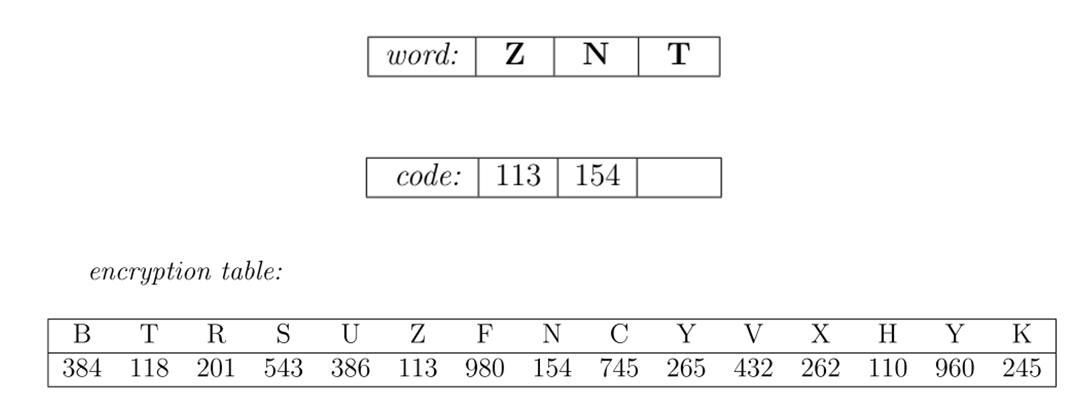
\includegraphics[scale=0.5]{Encryption_task}
	\label{task}
\end{figure}

Regardless of the treatment, all participants will make the encryption task in order to avoid potential confounders in the results. Before doing the paid encryption task, all participants will do a trial period, where they will be asked to solve precisely 10 puzzles of the task without being paid. When everybody successfully encrypts 10 words, the paid task will begin. Each participant will have 2 minutes to encrypt $e$ words. The payoff of the task will depend on achieving a minimum threshold of $e=7$. This threshold is based on the data provided by \citet{Benndorf2014} in which subjects did 9.37 words on average, and the standard deviation was 1.8; therefore, a minimum effort of 7 should be achieved by at least 90\% of the subjects.

In the baseline, participants who get a score of at least 7 words will earn $\Pi_{Re}$ whatever happens in the die-roll game, then the payoff of this stage  will be the following:
\[
\begin{cases} 
\Pi_{Re} & e \ge 7 \\
0 & otherwise
\end{cases}\]
In other words, in the baseline the real effort task and the die-roll game are independent. However, given that in the central treatment the task will determine the endowment, we rule out any possible dependency on these two tasks making participants in the baseline to play the encryption game as well.

\subsection{Die roll-game}
The die roll game will be the one presented before introduced by \citet{Fischbacher2013}. Participants will obtain a monetary payoff for lying $\Pi_L$ at the end of this task, that depends only on the report they make. Specifically, in the baseline participants will have a payoff of $rP$ if $r$ is less or equal to 
$5$ and $0$ otherwise; where $r$ is the reported value, and $P$ is the monetary payoff per unit reported.

\subsection{Treatments}

\subsubsection{Windfall endowment}

The first treatment of the experiment will include an endowment in the lying game. Participants will start with the effort task, and they will get paid in the same way as in the baseline. Then, we will tell them that they will be endowed with some ``windfall" money $\Pi_{Lo}$, and they will lose some part of it depending on the report they make on the die-roll. Therefore, subjects' payoff  will be:
\[\Pi_L =
\begin{cases} 
	\Pi_{Lo}-(r-5)L & r\leq 5 \\
	0 & r=6	
\end{cases}\]

Where $L$ is the monetary loss that depends on the reported number. For instance, if the participant reports that the number on the die was 5, then she will keep all the endowment. Conversely, if she reports that number that came up was a 1, she must return $4L$. The baseline and this treatment are equivalent as long as two conditions are fulfilled: 1) $\Pi_{Lo}=argmax \{rP\}$ and 2) $P=L$. If these two conditions hold, we have the same situation than in the baseline but with the difference that now people could lie for keeping the money, instead of gaining the money. Therefore, based on the literature we will expect that this endowment effect will imply that people will cheat more than in the baseline because they will have loss aversion what increases the cost of lying.


\begin{hypothesis}
Including the endowment effect will increase lying. Participants will lie more in the Windfall Endowment treatment than in the Baseline.
\end{hypothesis}

\subsubsection{Merited endowment}
In some real-world situations like taxes, people are required to report some private information that will have real consequences. Let take the example of the tax declaration as a benchmark. In this particular example, the fiscal authority could take taxes from people ex-ante, and in the next year, people need to hand in the tax declaration in order to get some money refunded. The other option is that the government wait until the end of the year and at that moment citizens should make their tax declaration, and they will have a bill according to their report. In practice, some countries use the first scheme, and others use the second scheme. 

We call this second treatment Merited Endowment. In this treatment, participants will start with real effort task, but with the following payoff scheme: 
\[
\begin{cases} 
\Pi_{Rm} & e \ge 7 \\
\Pi_{Lo} & otherwise
\end{cases}\]
 Where $\Pi_{Rm}=\Pi_{Re}+\Pi_{Lo}$. That is, they will earn a payoff $\Pi_{Rm} > \Pi_{Re}$ if the threshold is achieved, and the same endowment $\Pi_{Lo}$  if they do not.  In other words, $\Pi_{Lo}$ will be the flat wage for doing the task and $\Pi_{Rm}$ will be the bonus if they meet the goal. This setting is crucial in order to create the feeling in participants that they earned the endowment for the second task.
 
In this treatment, we use framing in order to create the feeling that the endowment was obtained in the real effort task. Participants will be told that an amount $\Pi_{Lo}$ obtained in the real effort task in the first stage will be now used in the die-roll game. In particular, participants will keep $(r-5)L$ from their endowment, i.e., the game will be the same as in windfall treatment, the only variation will be in terms of framing. We can then observe in Table \ref{desing} the comparison between treatments' payoff.

\begin{table}[]
	\caption{Payoff comparison between treatments}
\label{desing}
	\begin{tabular}{@{}llll@{}}
		\toprule
	 & \multicolumn{1}{c}{\begin{tabular}[c]{@{}c@{}}Real Effort \\ Task\end{tabular}}        & \multicolumn{1}{c}{\begin{tabular}[c]{@{}c@{}}Die-roll \\ game\end{tabular}}           & \multicolumn{1}{c}{\begin{tabular}[c]{@{}c@{}}Expected \\ Payoff\end{tabular}} \\ \midrule
		Baseline                                                      &  \begin{tabular}[c]{@{}l@{}}$\Pi_{Re}$ if $e \ge 7$\\ 0 otherwise\end{tabular}          & \begin{tabular}[c]{@{}l@{}}$\Pi_L = rP$ if $r\leq5$\\ 0 if $r=6$\end{tabular}          & $\Pi^*=\Pi_0+\Pi_{Re}+\Pi_L$                                                   \\ \midrule
		\begin{tabular}[c]{@{}l@{}}Windfall\\ Endowment\end{tabular} &  \begin{tabular}[c]{@{}l@{}}$\Pi_{Re}$ if $e \ge 7$\\ 0 otherwise\end{tabular}          & \begin{tabular}[c]{@{}l@{}}$\Pi_L = \Pi_{Lo}-(r-5)L$ if $r\leq5$\\ 0 if $r=6$\end{tabular} & $\Pi^*=\Pi_0+\Pi_{Re}+\Pi_L$                                                   \\ \midrule
		\begin{tabular}[c]{@{}l@{}}Merited \\ Endowment\end{tabular}  &  \begin{tabular}[c]{@{}l@{}}$\Pi_{Rm}$ if $e \ge 7$\\ $\Pi_{Lo}$ otherwise\end{tabular} & \begin{tabular}[c]{@{}l@{}}$\Pi_L = \Pi_{Lo}-(r-5)L$ if $r\leq5$\\ 0 if $r=6$\end{tabular} & $\Pi^*=\Pi_0+\Pi_{Re}+\Pi_L$                                                   \\ \bottomrule
	\end{tabular}

\small\raggedright Notice that there is a fixed show up fee, $\Pi_0$, that is the same across treatments.
\end{table}

Given that the variation between Windfall Endowment and Merited Endowment is only the framing about the origin of the endowment, if there are some differences, it should be attributed to the justification/fairness argument. Put another way, the difference between these two treatments will be because players could have some moral licensing for cheating since they could justify their unethical behavior saying that is fair to keep more money that they deserve. Therefore, we will expect that participants lie more in the treatment where the endowment is obtained by merit.

\begin{hypothesis}
	Participants will lie more in the Merit Endowment treatment than in the Windfall Endowment treatment.
\end{hypothesis}

\subsection{Procedures}

The experiment will be conducted in the Experimentallabor at Technical University Berlin and will last around 1 hour. The final profit of the participants will be at least 7 Euros, and the average will be around 15 Euros. The experiment will be programmed in O-Tree \citep{Chen2016}, and the recruitment will be done through ORSEE \citep{Greiner2015}. Subjects will participate in only one out of the three possible conditions. The game will be one-shot to avoid any learning concerns.

Using the data on \citet{Shalvi2011} on the treatment single-roll, we determine that we will need 35 subjects per treatment. This value was calculated for a power of 0.8 and a test size of 0.05, with an average of 3.97 and a standard deviation of 1.56. This sample size will allow us to detect average differences between treatments of at least 0.8 in the report, which is around half of a standard deviation. 

\section{Final Remarks}

The design presented in this paper seeks to understand the role of the endowment effect on the willingness to lie/tell the truth. To rule out possible confounders it isolates pure loss aversion from the endowment effect and fairness. The expected results are that loss aversion will increase lying. Besides, adding the feeling that they deserve the endowment will raise the lying even more. We built these hypotheses on the previous literature of endowment effect and fairness in ultimatum and dictator games. 

If the results are as expected it will imply, for instance, that institutions who are in charge of tax compliance should be careful and reduce the presence of the endowment effect. In general, it would imply that we should reduce the endowment effect when we need that people report private information.


\bibliography{Citations_Lying}
\bibliographystyle{apalike}


\end{document}
